\documentclass[conference]{IEEEtran}
\IEEEoverridecommandlockouts

\usepackage{cite}
\usepackage{tabularx}
\usepackage{booktabs}
\usepackage{amsmath,amssymb,amsfonts}
\usepackage{algorithmic}
\usepackage{graphicx}
\usepackage{textcomp}
\usepackage{xcolor}
\usepackage{url}


\def\BibTeX{{\rm B\kern-.05em{\sc i\kern-.025em b}\kern-.08em
    T\kern-.1667em\lower.7ex\hbox{E}\kern-.125emX}}

\begin{document}

\title{Formación de Equipos Múltiples: Un Enfoque MINLP para la Asignación de Personal a Proyectos}

\author{
    \IEEEauthorblockN{Ignacio Martínez Hernández}
    \IEEEauthorblockA{\textit{Doctorado Sistemas en Ingeniería} \\
        \textit{Optimización de Sistemas}\\
        \textit{Universidad de Talca}\\
        Curicó , Chile\\
        imartinez17@alumnos.utalca.cl}
}

\maketitle

\begin{abstract}
    La asignación de personal a múltiples proyectos es un desafío complejo en la gestión organizacional, que requiere un equilibrio entre las competencias técnicas y la cohesión social de los equipos. Este trabajo aborda el Problema de Formación de Múltiples Equipos (MTFP) mediante un modelo de Programación No Lineal Entera Mixta (MINLP). El modelo propuesto maximiza una métrica de eficiencia global que integra la afinidad sociométrica entre los individuos, los requerimientos de habilidades de cada proyecto y su prioridad estratégica. La implementación se realizó en Python utilizando Pyomo, con el solver Bonmin para la resolución. Los resultados experimentales sobre instancias sintéticas demuestran la validez y robustez del enfoque: el modelo encuentra soluciones óptimas validadas contra un método de fuerza bruta, escala eficientemente para problemas de tamaño realista y gestiona requerimientos inviables mediante un enfoque de relajación que identifica y cuantifica los déficits de habilidades, ofreciendo soluciones parciales accionables. Se concluye que el modelo es una herramienta de apoyo a la decisión práctica y efectiva para formar equipos más cohesivos y productivos.
    %Se aborda el Problema de Formación de Múltiples Equipos (MTFP) mediante un modelo de Programación No Lineal Entera Mixta (MINLP) que maximiza una métrica de eficiencia basada en afinidad sociométrica, requerimientos de habilidades y prioridad de proyectos. El modelo, implementado en Pyomo y resuelto con Bonmin, fue validado experimentalmente en instancias sintéticas, mostrando robustez, escalabilidad y capacidad para gestionar casos inviables mediante relajación. Se concluye que es una herramienta efectiva para la asignación de equipos más cohesivos y productivos.

\end{abstract}

\begin{IEEEkeywords}
    Formación de equipos, optimización, programación no lineal entera mixta, sociometría, Pyomo, Bonmin.
\end{IEEEkeywords}

\section{Introducción}
La formación de equipos multidisciplinarios es un desafío recurrente en la gestión organizacional, especialmente al ejecutar múltiples proyectos en áreas como ingeniería o desarrollo de software. Su eficiencia depende tanto de habilidades técnicas como de cohesión social \cite{gutierrez2016multiple}, y su asignación óptima requiere integrar competencias, relaciones interpersonales y restricciones operativas.

Este trabajo aborda el \textit{Problema de Formación de Múltiples Equipos (MTFP)} mediante un modelo MINLP que busca maximizar una métrica de eficiencia global considerando: (1) la afinidad social entre miembros, (2) el cumplimiento de requerimientos técnicos, y (3) la prioridad estratégica de proyectos. Sus contribuciones clave incluyen un enfoque cuantitativo para equilibrar aspectos técnicos y sociales, un mecanismo de relajación que permite encontrar soluciones parciales en casos inviables, y la validación experimental de escalabilidad en escenarios conflictivos.

El documento se estructura en secciones que abarcan la metodología adoptada, la formulación del modelo, el análisis de resultados, y consideraciones sobre la implementación y validación, además de conclusiones y propuestas para trabajos futuros.

\section{Metodología}

El enfoque propuesto para abordar el problema de formación de equipos multiples se divide en cuatro fases principales y conectadas entre sí:

\begin{enumerate}
    \item \textbf{Modelado del problema:} Se define formalmente el problema de asignación de recursos humanos a múltiples proyectos considerando la maximización de la afinidad social entre los miembros asignados. Este modelo incorpora variables y restricciones que aseguran asignaciones factibles y equilibradas, así como una función objetivo que mide la calidad social del equipo.

    \item \textbf{Generación de datos sintéticos:} Para evaluar y validar el modelo, se generan conjuntos de datos representativos de escenarios reales. Las relaciones sociales entre individuos y los requisitos de los proyectos se crean a partir de reglas controladas que simulan características típicas del contexto organizacional, asegurando diversidad en las instancias de prueba. Los datos se almacenan en formato JSON para facilitar su reutilización y análisis.

    \item \textbf{Implementación computacional:} Se emplea Pyomo\cite{pyomo_hart2011}, un lenguaje de modelado algebraico en Python, para construir el modelo de optimización. La solución se obtiene mediante el solver Bonmin\cite{bonmin_bonami2008}, capaz de manejar problemas de optimización no lineal entera mixta, lo cual es necesario debido a la inclusión de asignaciones de tiempo fraccionarias y discretas. El sistema permite configurar el modelo mediante archivos externos, lo que facilita la adaptación a diferentes tamaños y características del problema sin necesidad de modificar la estructura del código.

    \item \textbf{Resolución y análisis:} Se realizan experimentos numéricos sobre diversas instancias para evaluar la efectividad y escalabilidad del enfoque. Los resultados se analizan desde el punto de vista de la maximización de la afinidad social y la factibilidad de las soluciones. Se incluye un procedimiento de relajación para gestionar casos inviables, permitiendo identificar fortalezas y áreas de mejora del modelo.
\end{enumerate}


\section{Entorno Modelado y Consideraciones}

La formación de equipos en organizaciones que gestionan múltiples proyectos simultáneamente es un proceso complejo, influenciado por factores técnicos, humanos, económicos y temporales. Cada persona puede poseer múltiples habilidades y disponibilidad variable, y las interacciones sociales evolucionan con el tiempo. Además, existen restricciones presupuestarias, plazos de entrega y dependencias técnicas.

El modelo propuesto incorpora simplificaciones para hacerlo manejable:
\begin{itemize}
    \item Para simplificar el modelo, se asume que cada persona contribuye con una única habilidad predominante en el contexto de la asignación, aunque puede ser asignada parcialmente a varios proyectos.
    \item Se utiliza una \textit{matriz de afinidad social} \cite{gutierrez2016multiple} que refleja relaciones entre miembros, manteniéndose estática durante la asignación.
    \item Los proyectos se consideran independientes, sin compartir recursos ni tener dependencias.
\end{itemize}

Para capturar la prioridad de cada proyecto, se les asigna un \textit{peso} que sintetiza su relevancia estratégica. Aunque el modelo no incluye todas las complejidades, esta priorización garantiza que proyectos importantes impacten más en la solución final.

Es importante destacar que no se consideran múltiples habilidades por persona. También se limita el tiempo parcial a fracciones discretas (0\%, 50\%, 100\%) para evitar asignaciones poco realistas, transformando el problema en un modelo de Programación No Lineal Entera Mixta (MINLP).

Estas simplificaciones equilibran la fidelidad del modelo con la factibilidad computacional, permitiendo un enfoque en la interacción entre adecuación técnica y maximización de la afinidad social, aspectos centrales del problema de formación de equipos.

\section{Definición del Modelo}

Para abordar formalmente el desafío de asignar personal a múltiples proyectos de manera que se consideren tanto las competencias técnicas como la dinámica social, se propone un modelo de optimización matemática. Debido a la necesidad de incorporar decisiones sobre fracciones de tiempo discretas, el modelo resultante es de Programación No Lineal Entera Mixta (MINLP). El objetivo central de este modelo es ayudar a los gestores a tomar decisiones de asignación que no solo cubran las necesidades de habilidades de cada proyecto, sino que también fomenten la cohesión y la sinergia dentro de los equipos formados, ponderando estas asignaciones según la importancia estratégica de cada proyecto. Este enfoque busca una solución que equilibre la eficiencia técnica con un ambiente de colaboración favorable, reconociendo que ambos son cruciales para el éxito organizacional.

En organizaciones que gestionan múltiples proyectos simultáneos, la asignación eficiente de personas a proyectos es crucial para el éxito. Cada individuo aporta una habilidad específica necesaria para cumplir tareas, mientras que las relaciones sociales entre personas influyen en la dinámica y desempeño del equipo. Además, los proyectos tienen distintas prioridades estratégicas que deben ser consideradas en la asignación.

Para capturar estas realidades, el modelo utiliza los siguientes elementos:

\begin{itemize}
    \item \textbf{Individuos} (\(\mathcal{H}\)): representan a los empleados o colaboradores disponibles, cada uno con una habilidad predominante.
    \item \textbf{Proyectos} (\(\mathcal{P}\)): iniciativas o tareas que requieren ciertos recursos humanos para completarse.
    \item \textbf{Habilidades} (\(\mathcal{K}\)): conjunto universal de habilidades técnicas presentes en la organización, de las cuales cada proyecto puede requerir.
    \item \textbf{Matriz de afinidad social} (\(s_{ij}\)): refleja la calidad de la relación entre personas, que puede ser positiva (cooperación), negativa (conflicto) o neutra.
    \item \textbf{Grupos por habilidad} (\(Q_a\)): subconjunto de individuos \(i \in \mathcal{H}\) que poseen la habilidad específica \(a\).
    \item \textbf{Pesos de proyecto} (\(w_l\)): indican la importancia relativa o prioridad de cada proyecto dentro de la organización.
\end{itemize}


\begin{figure}[htbp]
    \centering
    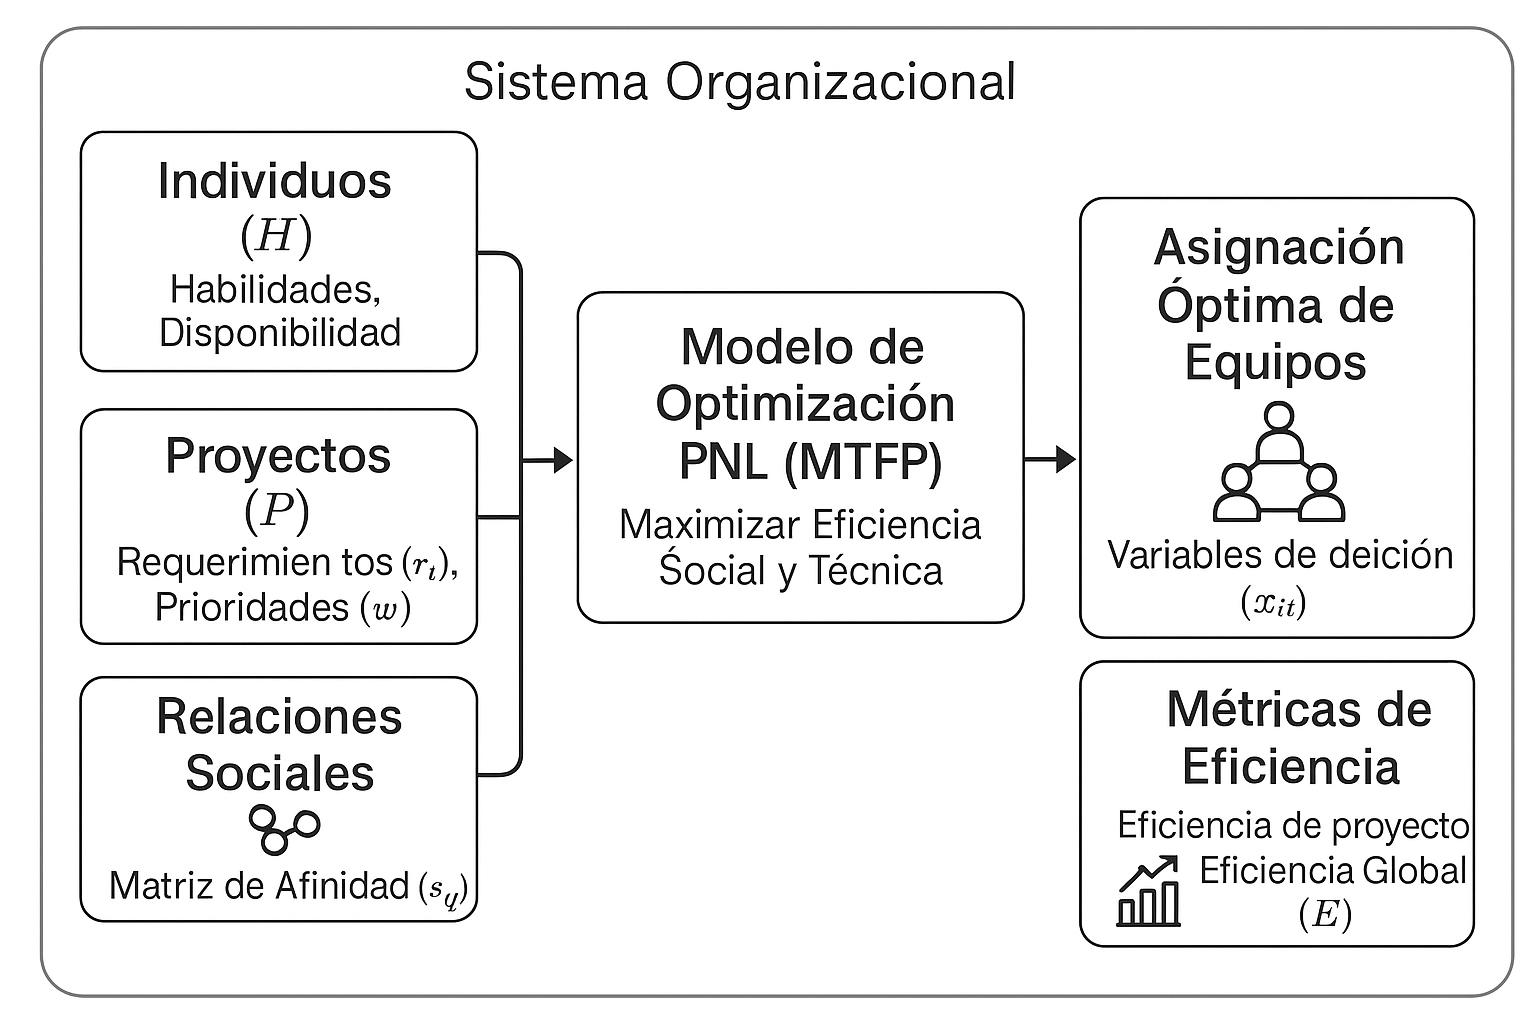
\includegraphics[width=0.8\linewidth]{diagrama_conceptual_mtfp.png}
    \caption{Modelo conceptual del Problema de Formación de Múltiples Equipos (MTFP), ilustrando sus componentes principales y flujos de información.}
    \label{fig:conceptual_model}
\end{figure}

\subsection{Conjuntos}
\begin{itemize}
    \item $\mathcal{H} = \{1, ..., n\}$: Individuos.
    \item $\mathcal{P} = \{1, ..., m\}$: Proyectos.
    \item $\mathcal{K} = \{1, ..., f\}$: Habilidades.
    \item $Q_a = \{i \in \mathcal{H} : \text{persona } i \text{ posee habilidad } a\}$, $\forall a \in \mathcal{K}$.
    \item $\mathcal{D}$: conjunto de fracciones de tiempo discretas permitidas para la asignación ($\{0.0, 0.5, 1.0\}$).
\end{itemize}


\subsection{Parámetros}
\[
    s_{ij} =
    \begin{cases}
        1,  & \text{si la afinidad social entre } i \text{ y } j \text{ es positiva}, \\
        0,  & \text{si no existe relación o es neutral},                              \\
        -1, & \text{si la afinidad social es negativa}.
    \end{cases}
\]
Se asume que la afinidad de una persona consigo misma es positiva, es decir, \(s_{ii} = 1, \forall i \in \mathcal{H}\).

\begin{itemize}
    \item $r_{al} \in \mathbb{R}$: cantidad mínima de dedicación (en personas) con habilidad $a$ requerida en el proyecto $l$.
    \item $w_l \in [0,1]$: peso o prioridad del proyecto $l$, con $\sum_{l \in \mathcal{P}} w_l = 1$.
\end{itemize}

\subsection{Variable de decisión}

\begin{itemize}
    \item \(x_{il} \in \mathcal{D}\): fracción del tiempo total del individuo \(i\) asignado al proyecto \(l\), donde \(\mathcal{D}\) es el conjunto de fracciones discretas permitidas.
\end{itemize}

\subsection{Función objetivo}

A continuación, se detalla la función objetivo que integra estos elementos para maximizar la eficiencia global de la asignación.
El modelo maximiza una métrica de eficiencia global que pondera la cohesión social de los equipos y la prioridad de los proyectos. La eficiencia de cada proyecto \(l\) se define como:
\begin{equation}
    e_l = \frac{1}{2} \left( 1 + \frac{\sum_{i,j \in \mathcal{H}} s_{ij} x_{il} x_{jl}}{\left(\sum_{a \in \mathcal{K}} r_{al}\right)^2} \right)
    \label{eq:efficiency_project_updated}
\end{equation}
donde el numerador mide la afinidad social ponderada por la participación conjunta, y el denominador normaliza respecto al tamaño del proyecto. Así, \(e_l\) queda acotado entre 0 y 1.

La función objetivo global es:
\begin{equation}
    \max E = \sum_{l \in \mathcal{P}} w_l \cdot e_l
    \label{eq:objective_total_updated}
\end{equation}
priorizando proyectos según su importancia relativa.

\subsection{Restricciones}
El modelo está sujeto a un conjunto de restricciones que reflejan las limitaciones y requerimientos operativos del mundo real en la asignación de personal:

\begin{align}
    \sum_{l \in \mathcal{P}} x_{il}  &\leq 1, && \forall i \in \mathcal{H} \label{eq:constraint_capacity_updated} \\
    \sum_{i \in Q_a} x_{il}          &= r_{al}, && \forall a \in \mathcal{K}, \forall l \in \mathcal{P} \label{eq:constraint_skills_updated}
\end{align}

\begin{equation}
    x_{il} \in \mathcal{D}, \quad \forall i \in \mathcal{H}, \forall l \in \mathcal{P}
    \label{eq:constraint_discrete}
\end{equation}

\begin{itemize}
    \item \textbf{Restricción de Capacidad Individual (Ecuación \ref{eq:constraint_capacity_updated})}: Esta restricción asegura que la asignación total de tiempo de un individuo \(i\) a todos los proyectos (\(\sum_{l \in \mathcal{P}} x_{il}\)) no exceda su disponibilidad total, que se normaliza a 1 (representando el 100\% de su tiempo laboral disponible). En el mundo real, esto significa que una persona no puede ser asignada a más trabajo del que puede realizar. Limita la sobrecarga de los individuos y refleja la finitud de los recursos humanos.

    \item \textbf{Restricción de Requerimientos de Habilidad por Proyecto (Ecuación \ref{eq:constraint_skills_updated})}: Esta restricción garantiza que para cada proyecto \(l\) y cada habilidad \(a\), la suma de las fracciones de tiempo de todas las personas (\(i \in Q_a\)) que poseen dicha habilidad y son asignadas al proyecto, sea exactamente igual a la cantidad requerida (\(r_{al}\)). Se optó por una igualdad estricta en lugar de una desigualdad (\(\geq\)) por una razón fundamental: evitar la sobreasignación de recursos. Si se permitiera una asignación mayor o igual, la función objetivo, en su afán por maximizar la afinidad social, tendería a asignar a todas las personas disponibles con afinidades positivas, incluso si exceden con creces los requerimientos técnicos. La igualdad impone un principio de eficiencia de recursos, asegurando que los equipos se dimensionen precisamente según las necesidades, lo que se alinea mejor con objetivos de control de costos y gestión práctica. Esta rigidez, sin embargo, es una de las principales causas de inviabilidad del modelo, lo que justifica la posterior introducción de un mecanismo de relajación.

    \item \textbf{Restricción de Discreción en la Asignación (Ecuación \ref{eq:constraint_discrete})}: La restricción \(x_{il} \in \mathcal{D}\) asegura que las fracciones de tiempo asignadas a cada individuo en cada proyecto solo pueden tomar valores del conjunto discreto permitido, reflejando la naturaleza realista y operativa de la asignación de recursos en la organización.

\end{itemize}

Estas restricciones son fundamentales para garantizar que la solución del modelo sea factible y refleje las realidades operativas de la organización. La primera asegura que no se asignen más recursos humanos de los disponibles, mientras que la segunda garantiza que cada proyecto cuente con el personal necesario para cumplir sus objetivos técnicos.

\subsection{Relajación para Casos Inviables}
\label{sec:relaxation_infeasible}

En situaciones donde el modelo estricto no tiene solución factible, se introduce una relajación que permite déficits en los requerimientos de habilidades. Para ello, se agregan variables de holgura \(\delta_{al} \geq 0\) en la restricción de requerimientos:
\begin{equation}
    \sum_{i \in Q_a} x_{il} + \delta_{al} = r_{al}, \quad \forall a \in \mathcal{K}, \forall l \in \mathcal{P}
    \label{eq:constraint_skills_relaxed}
\end{equation}
La función objetivo se modifica para penalizar estos déficits:
\begin{equation}
    \max E_{\text{relajado}} = \left( \sum_{l \in \mathcal{P}} w_l \cdot e_l \right) - \lambda \sum_{l \in \mathcal{P}} \sum_{a \in \mathcal{K}} \delta_{al}
    \label{eq:objective_total_relaxed}
\end{equation}
donde \(\lambda\) es un coeficiente de penalización suficientemente grande para forzar al solver a minimizar el déficit.

Esta relajación permite al modelo encontrar soluciones parciales en casos inviables, identificando déficits de habilidades y ofreciendo una métrica de eficiencia que considera tanto la afinidad social como la capacidad técnica.

\section{Análisis del Modelo y Justificación de Simplificaciones}

El modelo MTFP presentado constituye una abstracción matemática del complejo proceso real de asignación de personal. Para lograr tratabilidad computacional, incorpora simplificaciones clave que analizamos a continuación.

\subsection{Naturaleza Estática}
Mientras la formación real de equipos es dinámica (con relaciones y prioridades cambiantes), el modelo proporciona una solución óptima para parámetros fijos en un momento dado. Esta aproximación estática permite obtener soluciones eficientes, sirviendo como punto de partida para asignaciones que pueden reevaluarse periódicamente.

\subsection{Parámetros Fijos}
La matriz de afinidad social ($s_{ij}$) y pesos de proyecto ($w_l$) permanecen constantes durante la optimización, aunque en la práctica evolucionan. Esta simplificación es necesaria para mantener la tratabilidad del modelo, evitando la complejidad de enfoques dinámicos o de simulación. En aplicaciones reales, los parámetros pueden actualizarse entre ejecuciones.

\subsection{Retroalimentación Externa}
El modelo carece de mecanismos internos de ajuste continuo, ya que está diseñado como herramienta de optimización para estados específicos del sistema. Los procesos de monitorización y corrección ocurren externamente, pudiendo informar nuevas ejecuciones con parámetros actualizados.

\subsection{Implicaciones Prácticas}
Estas simplificaciones posicionan al modelo como:
\begin{itemize}
\item Un sistema de \textit{apoyo a decisiones} para momentos específicos
\item Una solución robusta al problema combinatorio de asignación
\item Un balance entre rigor matemático y aplicabilidad operativa
\end{itemize}

Los resultados deben interpretarse como recomendaciones que los gestores pueden integrar dentro de procesos organizacionales más amplios y dinámicos.

\section{Implementación Computacional}

El modelo se implementó en \textbf{Pyomo} \cite{pyomo_hart2011}, aprovechando su flexibilidad para problemas MINLP y su integración con el solver \textbf{Bonmin} \cite{bonmin_bonami2008}. La configuración y los datos se gestionan mediante archivos JSON, permitiendo adaptar fácilmente el modelo a distintos escenarios. El flujo de trabajo consiste en: carga o generación de datos, construcción del modelo, resolución con Bonmin y almacenamiento de resultados. El código completo está disponible públicamente\footnote{\url{https://github.com/DarkNacho/Multiple-Team-Formation}}.

Esta implementación permite adaptar el modelo a diferentes escenarios organizacionales mediante simple modificación de los archivos de configuración, sin necesidad de alterar el núcleo algorítmico.

\section{Resultados y Discusión}

Al interpretar la métrica de eficiencia del proyecto $e_l$, definida en la Ecuación \ref{eq:efficiency_project_updated}, es importante considerar una sutileza relacionada con la matriz de afinidad social $s_{ij}$. Como se describió anteriormente, un valor de $e_l=0.5$ se interpreta como un punto de cohesión neutra, donde las afinidades positivas y negativas se cancelan. Sin embargo, es una convención común o una implicación de la definición de $s_{ij}$ que la afinidad de un individuo consigo mismo, $s_{ii}$, sea 1. Si este es el caso, la diagonal de la matriz de afinidad contribuye positivamente a la suma $\sum_{i,j \in \mathcal{H}} s_{ij} x_{il} x_{jl}$.

Específicamente, el término $\sum_{i,j \in \mathcal{H}} s_{ij} x_{il} x_{jl}$ en el numerador de $e_l$ incluye la suma de los cuadrados de las asignaciones ponderadas por la auto-afinidad, es decir, $\sum_{i \in \mathcal{H}} s_{ii} x_{il}^2$. Si $s_{ii}=1$ para todo $i$, este componente es $\sum_{i \in \mathcal{H}} x_{il}^2$, que es inherentemente no negativo. Para que la eficiencia $e_l$ sea exactamente 0.5, la suma total $\sum_{i,j \in \mathcal{H}} s_{ij} x_{il} x_{jl}$ debe ser cero. Esto implica que la suma de las afinidades interpersonales (es decir, los términos donde $i \neq j$) no solo debe ser cero por sí misma, sino que debe ser suficientemente negativa para contrarrestar el término positivo $\sum_{i \in \mathcal{H}} x_{il}^2$.

En consecuencia, un equipo donde todas las relaciones \textit{interpersonales} son estrictamente neutras (es decir, $s_{ij}=0$ para todo $i \neq j$), y asumiendo $s_{ii}=1$, resultaría en un valor de $e_l$ ligeramente superior a 0.5, dado por:
\[ e_l = \frac{1}{2} \left( 1 + \frac{\sum_{i \in \mathcal{H}} x_{il}^2}{\left(\sum_{a \in \mathcal{K}} r_{al}\right)^2} \right) \]
Esta consideración no invalida la utilidad de $e_l$ como un indicador de la cohesión social del equipo, ni el rango de $[0,1]$. Simplemente refina la interpretación del punto $e_l=0.5$: este valor representa un estado donde las interacciones sociales negativas entre distintos miembros del equipo son lo suficientemente fuertes como para anular tanto las interacciones positivas entre otros miembros como la contribución basal positiva derivada de las auto-afinidades. La escala sigue siendo efectiva para comparar la cohesión relativa entre diferentes configuraciones de equipos. En lo que respecta al límite inferior de la escala, $e_l=0$, este se alcanzaría si el término de afinidad social total, $\sum_{i,j \in \mathcal{H}} s_{ij} x_{il} x_{jl}$, fuese igual a $-\left(\sum_{a \in \mathcal{K}} r_{al}\right)^2$. Considerando la contribución inherentemente positiva de las auto-afinidades (asumiendo $s_{ii}=1$), para que $e_l$ llegue a cero, la suma de las afinidades interpersonales negativas ($\sum_{i \neq j} s_{ij} x_{il} x_{jl}$) debe ser excepcionalmente fuerte, superando no solo las afinidades interpersonales positivas sino también la suma de $\sum_{i \in \mathcal{H}} x_{il}^2$. De hecho, para equipos muy pequeños (uno o dos miembros), incluso si todas las afinidades interpersonales fuesen -1 (y $s_{ii}=1$), el valor de $e_l$ no podría ser 0 (y, de hecho, se mantendría $\geq 0.5$) si existen requerimientos de proyecto ($\sum_{a \in \mathcal{K}} r_{al} > 0$), ya que la contribución positiva de las auto-afinidades no es superada en tal medida. Sin embargo, para equipos más grandes (tres o más miembros), es teóricamente posible que $e_l$ alcance el valor 0 si las interacciones negativas son suficientemente intensas y generalizadas. En la práctica, un valor de $e_l$ cercano a 0 siempre indicará un nivel de conflicto social extremadamente alto y perjudicial para el proyecto.

Este comportamiento teórico se confirma en los experimentos de robustez. Como se observa en la Tabla \ref{tab:robustez}, incluso en un escenario extremo donde el 100\% de las afinidades interpersonales son negativas, la eficiencia global resultante es de 22.22\%, un valor marcadamente superior a cero. Este resultado ilustra cómo la contribución basal positiva de las auto-afinidades ($s_{ii}=1$) impide que la eficiencia colapse a 0, incluso bajo un conflicto generalizado, ya que el modelo debe cumplir con los requerimientos técnicos del proyecto.

\par Para evaluar la efectividad, robustez y escalabilidad del modelo MINLP propuesto, se diseñó y ejecutó un plan de pruebas exhaustivo. Los experimentos se realizaron sobre un conjunto de instancias sintéticas, generadas para simular diversos escenarios organizacionales. A continuación, se presentan y discuten los resultados obtenidos en cada una de las baterías de pruebas.

\subsection{Validación de Correctitud}
Para verificar la correctitud del modelo MINLP, la primera fase de experimentación consistió en comparar sus resultados con los de un método de referencia que garantiza la optimalidad: un algoritmo de fuerza bruta. Este algoritmo explora sistemáticamente todas las asignaciones posibles para encontrar la solución óptima global. Se utilizaron instancias de tamaño reducido, donde la exploración exhaustiva es computacionalmente factible.

Los resultados, resumidos en la Tabla \ref{tab:correctitud}, muestran una coincidencia exacta entre la eficiencia global óptima encontrada por el solver Bonmin y la obtenida por el método de fuerza bruta en todos los casos de prueba, incluyendo escenarios con afinidades negativas.

\begin{table}[htbp]
    \centering
    \caption{Comparación de resultados entre el solver y fuerza bruta para validación.}
    \label{tab:correctitud}
    \begin{tabularx}{\linewidth}{@{}lccc@{}}
        \toprule
        \textbf{Instancia}               & \textbf{Eficiencia Global} & \textbf{Eficiencia Global} \\
        (Personas/Proyectos/Habilidades) & \textbf{Fuerza Bruta}      & \textbf{Solver}            \\
        \midrule
        2p / 1pr / 1sk (afin. pos)       & 100.00\%                   & 100.00\%                   \\
        3p / 2pr / 2sk (afin. mix)       & 100.00\%                   & 100.00\%                   \\
        4p / 2pr / 2sk (afin. nega)      & 75.00\%                    & 75.00\%                    \\
        6p / 1pr / 2sk (excedente)       & 75.00\%                    & 75.00\%                    \\
        \bottomrule
    \end{tabularx}
\end{table}

La perfecta correspondencia en los valores de la función objetivo, así como en las asignaciones de variables de decisión, confirma que el modelo está formulado correctamente y que el solver es capaz de encontrar la solución óptima global para problemas de baja dimensionalidad. Esta validación inicial es un paso crucial antes de proceder a evaluar la escalabilidad y el comportamiento del modelo en instancias de mayor tamaño.

\subsection{Análisis de Escalabilidad}
Se evaluó el comportamiento del modelo frente a instancias de tamaño creciente para medir su escalabilidad. Se generaron problemas con un número de personas desde 10 hasta 100, con un aumento proporcional en el número de proyectos y habilidades. Los resultados se resumen en la Tabla \ref{tab:escalabilidad}.

\begin{table}[htbp]
    \centering
    \caption{Resultados de las pruebas de escalabilidad.}
    \label{tab:escalabilidad}
    \begin{tabularx}{\linewidth}{@{}lccc@{}}
        \toprule
        \textbf{Instancia}               & \textbf{Eficiencia} & \textbf{Tiempo (s)} \\
        (Personas/Proyectos/Habilidades) & \textbf{Global}     &                     \\
        \midrule
        10p / 2pr / 2sk                  & 81.90\%             & 0.22                \\
        20p / 5pr / 4sk                  & 75.11\%             & 0.84                \\
        30p / 5pr / 4sk                  & 60.22\%             & 5.05                \\
        50p / 10pr / 8sk                 & 73.65\%             & 45.11               \\
        100p / 10pr / 8sk                & 67.86\%             & 622.19              \\
        \bottomrule
    \end{tabularx}
\end{table}

Como era de esperar, el tiempo de resolución aumenta de forma no lineal con el tamaño del problema, lo cual es característico de los problemas MINLP. Para la instancia más grande, con 100 personas, el modelo tardó poco más de 10 minutos en encontrar la solución óptima. Este resultado es prometedor, ya que demuestra que el modelo es capaz de resolver problemas de tamaño realista en un tiempo razonable.

\subsection{Impacto de la Discretización del Tiempo}
Se analizó cómo la granularidad de las fracciones de tiempo permitidas (\(\mathcal{D}\)) afecta la solución y el rendimiento. Se ejecutó la misma instancia (6 personas, 2 proyectos, 2 habilidades) con tres conjuntos de fracciones distintos. La Tabla \ref{tab:discretizacion} compara los resultados obtenidos por el solver Bonmin y el algoritmo de fuerza bruta.

\begin{table}[htbp]
    \centering
    \caption{Impacto de la discretización del tiempo en una instancia de 6p/2pr/2sk.}
    \label{tab:discretizacion}
    \begin{tabularx}{\linewidth}{@{}lccc@{}}
        \toprule
        \textbf{Fracciones Permitidas (\(\mathcal{D}\))} & \textbf{Eficiencia} & \textbf{Tiempo}     & \textbf{Tiempo}           \\
                                                         & \textbf{Global}     & \textbf{Solver (s)} & \textbf{Fuerza Bruta (s)} \\
        \midrule
        \{0, 1\}                                         & 88.89\%             & 0.18                & 0.04                      \\
        \{0, 0.5, 1\}                                    & 88.89\%             & 0.13                & 3.56                      \\
        \{0, 0.25, 0.5, 0.75, 1\}                        & 88.89\%             & 0.13                & 1407.97                   \\
        \bottomrule
    \end{tabularx}
\end{table}

Los resultados muestran que, para esta instancia particular, la eficiencia global óptima fue la misma en todos los escenarios, indicando que la solución óptima no requería asignaciones de tiempo parciales. Sin embargo, el análisis del tiempo de cómputo revela una diferencia crucial: mientras que el tiempo del solver se mantuvo estable y bajo, el tiempo del algoritmo de fuerza bruta creció de manera exponencial. Al aumentar la granularidad, el espacio de búsqueda para la fuerza bruta se expandió drásticamente, llevando el tiempo de ejecución de 0.04 segundos a más de 23 minutos.

Este experimento subraya dos puntos importantes: primero, la capacidad del modelo para manejar fracciones de tiempo finas es una característica clave para problemas más complejos donde las asignaciones parciales podrían ser necesarias para alcanzar la optimalidad. Segundo, demuestra la clara superioridad computacional del solver MINLP sobre un método de búsqueda exhaustiva, siendo indispensable para resolver problemas de tamaño realista de manera eficiente.

\subsection{Robustez ante Afinidades Negativas}
Para medir la capacidad del modelo de gestionar conflictos interpersonales, se crearon instancias con una proporción creciente de afinidades negativas, desde un 50\% hasta un 100\%. Los resultados (Tabla \ref{tab:robustez}) muestran que la eficiencia global disminuye drásticamente a medida que aumenta la proporción de afinidades negativas. Esto ocurre porque el modelo se ve forzado a asignar personas con conflictos para cumplir con los requerimientos técnicos de los proyectos.

\begin{table}[htbp]
    \centering
    \caption{Impacto de afinidades negativas en una instancia de 6p/2pr/2sk.}
    \label{tab:robustez}
    \begin{tabularx}{\linewidth}{@{}lcccc@{}}
        \toprule
        \textbf{Proporción Negativas} & \textbf{Eficiencia Global} \\
        \midrule
        50\%                          & 55.56\%                    \\
        60\%                          & 38.89\%                    \\
        80\%                          & 33.33\%                    \\
        90\%                          & 22.22\%                    \\
        100\%                         & 22.22\%                    \\
        \bottomrule
    \end{tabularx}
\end{table}

Este comportamiento demuestra que el modelo es sensible a la estructura social y penaliza fuertemente las configuraciones de equipos con alta conflictividad, tal como se esperaba. Para validar la calidad de la solución, el caso con 50\% de afinidades negativas se verificó mediante fuerza bruta, confirmando que la eficiencia del 55.56\% es óptima. Sin embargo, la fuerza bruta requirió 1441.19 segundos (aprox. 24 minutos) para encontrarla, en contraste con los 0.28 segundos del solver. Este resultado subraya la capacidad del modelo para encontrar soluciones óptimas de manera eficiente incluso en escenarios de alta conflictividad.

\subsection{Sensibilidad a la Prioridad de Proyectos}
Se evaluó si el modelo responde correctamente a los pesos (\(w_l\)) asignados a los proyectos. Se configuró una instancia con dos proyectos, variando sus pesos relativos. Los resultados se muestran en la Tabla \ref{tab:sensibilidad}.

\begin{table}[htbp]
    \centering
    \caption{Sensibilidad a la prioridad de proyectos en una instancia de 6p/2pr/2sk.}
    \label{tab:sensibilidad}
    \begin{tabularx}{\linewidth}{@{}lcccc@{}}
        \toprule
        \textbf{Pesos (P1, P2)} & \textbf{Eficiencia P1} & \textbf{Eficiencia P2} & \textbf{Eficiencia Global} \\
        \midrule
        (80\%, 20\%)            & 88.89\%                & 77.78\%                & 86.67\%                    \\
        (95\%, 5\%)             & 88.89\%                & 77.78\%                & 88.33\%                    \\
        \bottomrule
    \end{tabularx}
\end{table}

En ambos experimentos, el modelo asignó el mismo conjunto de personas a cada proyecto. Aunque la asignación no cambió, el resultado demuestra que el modelo prioriza correctamente, ya que la eficiencia global ponderada aumenta conforme se asigna mayor peso al proyecto con el equipo más cohesivo (Proyecto 1). La asignación de personas no varió porque ya era óptima para ambos proyectos; el cambio en los pesos simplemente re-evalúa la importancia de cada equipo en la función objetivo global.

\subsection{Gestión de Casos Inviables y Relajación del Modelo}

Finalmente, se probó la robustez del modelo ante escenarios sin solución factible. Para ello, se implementó el modelo relajado descrito en la Sección~\ref{sec:relaxation_infeasible}. Los resultados (Tabla~\ref{tab:infeasible}) muestran la eficiencia global alcanzada y el déficit total de habilidades no cubiertas.

Los resultados de las pruebas sobre instancias inviables (Tabla \ref{tab:infeasible}) confirman la efectividad de este enfoque. El modelo estricto identifica correctamente la inviabilidad, y el modelo relajado procede a encontrar una solución óptima parcial. La tabla detalla la eficiencia global alcanzada a pesar de la inviabilidad y el déficit total, que representa la suma de todas las unidades de habilidad (medidas en personas-equivalente) que no pudieron ser asignadas para cumplir con los requerimientos originales de los proyectos.

\begin{table}[htbp]
    \centering
    \caption{Resultados del modelo relajado sobre instancias inviables.}
    \label{tab:infeasible}
    \begin{tabularx}{\linewidth}{@{}lrrr@{}}
        \toprule
        \textbf{Instancia}               & \textbf{Eficiencia Global} & \textbf{Déficit Total} \\
        (Personas/Proyectos/Habilidades) &                            &                        \\
        \midrule
        4p / 2pr / 2sk                   & 66.39\%                    & 3.0                    \\
        6p / 2pr / 2sk                   & 54.32\%                    & 12.0                   \\
        10p / 3pr / 2sk                  & 79.93\%                    & 1.5                    \\
        15p / 4pr / 5sk                  & 66.80\%                    & 3.0                    \\
        \bottomrule
    \end{tabularx}
\end{table}

\section{Conclusiones y Trabajo Futuro}
Este trabajo ha presentado un modelo de Programación No Lineal Entera Mixta (MINLP) para el Problema de Formación de Múltiples Equipos (MTFP), que integra de manera efectiva los requerimientos técnicos de los proyectos con la cohesión social de los equipos, ponderada por la prioridad estratégica de cada proyecto. La implementación, utilizando Pyomo y el solver Bonmin, ha demostrado ser una herramienta robusta y eficaz para abordar este complejo problema de asignación.

Los resultados experimentales validan la efectividad y aplicabilidad del modelo. Se ha confirmado su correctitud al replicar las soluciones óptimas de un método de fuerza bruta en instancias pequeñas. El análisis de escalabilidad muestra que el modelo es capaz de resolver problemas de tamaño realista (100 personas) en tiempos computacionales razonables, lo que subraya su viabilidad práctica. Los experimentos de robustez demostraron que el modelo gestiona adecuadamente los conflictos interpersonales y es sensible a la prioridad de los proyectos.

Una de las contribuciones más significativas de este trabajo es la gestión de casos inviables. El modelo no solo identifica la inviabilidad, sino que, a través de un mecanismo de relajación de dos etapas, proporciona una solución parcial óptima. Esta solución cuantifica con precisión el déficit de habilidades para cada proyecto, ofreciendo información de gran valor para la toma de decisiones estratégicas, como la contratación de personal, la capacitación o la renegociación del alcance de los proyectos. Esta capacidad transforma el modelo de una simple herramienta de asignación a un sistema de apoyo diagnóstico para la planificación de recursos.

Como trabajo futuro, se proponen varias líneas de extensión. Primero, se podría enriquecer el modelo para incluir habilidades secundarias en los individuos y penalizar la sobreasignación de recursos. Segundo, se propone explorar una reinterpretación de la matriz de afinidad ($s_{ij}$) para capturar factores más complejos, como el bienestar individual ($s_{ii}$) o la compatibilidad profesional efectiva. Tercero, el mecanismo de relajación podría sofisticarse, permitiendo penalizaciones diferenciadas por proyecto o habilidad, o incluso la exclusión automática de proyectos si su déficit supera un umbral crítico. Finalmente, se podría evaluar el rendimiento del modelo con otros solvers MINLP o desarrollar heurísticas específicas para resolver instancias de muy grande escala de manera más rápida, aunque potencialmente subóptima.


\begin{thebibliography}{00}

    \bibitem{gutierrez2016multiple}
    J. H. Gutiérrez, C. A. Astudillo, P. Ballesteros-Pérez, D. Mora-Melià, \& A. Candia-Véjar,
    \textit{The multiple team formation problem using sociometry},
    Computers \& Operations Research, vol. 75, pp. 150--162, 2016. DOI: \texttt{10.1016/j.cor.2016.05.012}.

    \bibitem{pyomo_hart2011}
    W. E. Hart, J. P. Watson, \& D. L. Woodruff,
    \textit{Pyomo: modeling and solving mathematical programs in Python},
    Mathematical Programming Computation, vol. 3, no. 3, pp. 219--260, 2011. DOI: \texttt{10.1007/s12532-011-0026-8}.


    \bibitem{bonmin_bonami2008}
    Pierre Bonami, Lorenz T. Biegler, Andrew R. Conn, Gérard Cornuéjols, Ignacio E. Grossmann, Carl D. Laird, Jon Lee, Andrea Lodi, François Margot, Nicolas Sawaya, Andreas Wächter,
    \textit{An algorithmic framework for convex mixed integer nonlinear programs},
    Discrete Optimization, vol. 5, no. 2, pp. 186--204, May 2008. DOI: \texttt{10.1016/j.disopt.2006.10.011}.

\end{thebibliography}

\end{document}